\chapter{Fabrication \& Sensing of Input Devices}


\begin{quote}
In addition to the profound repercussions these technologies
will likely have on the manufacturing industry, the
democratization they enable promises to unleash creativity
and innovation at a level comparable to those brought about
by the personal computer and the internet.

--- Catarina Mota, \emph{The Rise of Personal Fabrication}
\end{quote}

Our goal is to enable simple construction of input devices. The route that we choose to take for this is digital fabrication, as it allows us to create prototypes whose properties we can predict and thereby sense. In essence, each input device takes a user action and transforms it through some type of mechanism. The mechanism is constructed from materials with various properties, and the combination of materials properties, user interaction, and transformative mechanism lead to a senseable change; all that's left is to select a sensor that can detect it. Thanks to digital fabrication, can use our knowledge of the mechanism to be fabricated along with its predicted properties to make sensing easier.  For example, perhaps we desire to sense a user's physical movement (e.g., pushing, sliding, or turning). Some processes can create tine structures (cantilevered beams); when struck, these tines vibrate at frequencies determined by their geometry and material, so we place these tines under a printed mechanism that translates a user's action into tine plucks. Finally, we can sense the tines' vibrations with a microphone, and decode the signal for use in our application. We need not train the algorithm beyond giving it the digital design file---we can predict the tines' vibrational frequency from that and our knowledge of our selected material's properties.

Stu Card, et al., describe the design space of input devices using movement operators (linear/rotary, absolute/relative, movement/force) and composition operators (merge, layout, connect); they represent each input device as a tuple $(M, In, S, R, Out, W)$ detailing user manipulation, the input space, the device's current state, the resolution or mapping function from input space to output space, the output space, and ``additional aspects of how a device works'' \cite{card-input}. Since our focus is on the \emph{construction} of such input devices, we refer the interested reader to Card, et al.,'s description of user inputs and possible mechanisms therefor. This chapter will describe the spaces of materials properties, modern digital fabrication machines, and sensors. Further, we will discuss potential ``links'' between these, as in the tine example above.

\section{Definitions}

First, we briefly define words and machines that will be discussed in this chapter and the remainder of the thesis.

\emph{additive fabrication} : in additive fabrication, material is deposited and a shape is built up.

\emph{subtractive fabrication} : a subtractive fabrication process removes material to create a form. Excess material may be reused in another project or discarded.

\emph{3D printer} : a 3D printer is one of a class of machines that additively create a three-dimenstional model from one or more materials.

\emph{FFF} : FFF (fused-filament fabrication) 3D printers lay down material by melting and depositing a filament in a precise pattern.

\emph{model material} : model material is the substrate that the final object is made from

\emph{support material} : many modern 3D printers are capable of laying two types of materials, model material and a secondary, sacrificial material that can support overhangs in the model while printing, then be removed.

\emph{SLA} : SLA (stereolithography) printers use a bath of UV-curable polymer and a controllable UV laser. The laser "draws" each layer on the polymer, causing photopolymerization where it strikes. Excess material is simply poured out for reuse.

\emph{SLS} : SLS (selective laser sintering) 3D printers contain a bed of material (e.g., metal powder) which is compacted and formed into a solid mass of material by heat and/or pressure without melting to the point of liquefaction. Excess material can be brushed off and reused.

\emph{Polyjet} : Polyjet printers have print heads similar to those of inkjet printers which sweep across the build area depositing material. Following the printer head is a UV light, which cures deposited material droplets.

\emph{vinyl cutter} : a vinyl cutter subtractively processes 2D materials with a 2-axis knife blade, cutting patterns into them. Vinyl cutters are typically used for thin, flexible materials.

\emph{laser cutter} : a laser cutter has a 2-axis laser for processing flat materials. Laser cutters can cut or engrave into materials, and are often used for rigid materials $<\frac{1}{4}$ inch thick. Some have rotary attachments for engraving on circular surfaces like the outside of a glass.

\emph{CNC router} : a CNC router uses a 3-axis rotary mill to cut through thick, rigid materials, like wood or certain metals. Some CNC routers are portable and can attach to many materials, while some are stationary with beds into which material is loaded.

\emph{CNC mill} : a CNC mill is a multi-axis machine which subtractively creates a 3D shape from a block of material, usually metal or wood.

\section{Digital Fabrication}

Digital fabrication machines are those which can take as input a digital design file, in 2D, 2.5D, or 3D, and output a physical realization of that design. A design created in a computer-aided design (CAD) tool is processed by a computer-aided manufacturing (CAM) tool to create machine instructions to generate the object. This workflow stands in contrast to traditional crafting techniques (which do not require machine code) as well as traditional manufacturing techniques (which require ``tooling'' for each design created). The true power of digital fabrication lies in its ability to create unique objects on each machine run \emph{without} the extensive setup and tooling necessary to change the product created by, for example, an injection moulding machine. This comes with the blessing and curse that each instance of an object costs as much to manufacture as the one before it, but allows for variations between instances without additional cost. For example, even makers can now create custom 3D printed replacement joints and prosthetics that fit particular bodies, e.g., a new hand for a young girl who wants to play on the playground \cite{myers-sophie}.

The joint interests of industry, academia, and hobbyist makers have led to a flourishing ecosystem of digital fabrication and rapid prototyping (RP) machines. These machines describe a continuum from simple vinyl cutters that can subtractively create 2-dimensional stickers to sophisticated multi-material 3D printers that can create multicolor and conductive designs where the designer has full 3D control over the geometry of the object. These machines allow their manufactured products to achieve various material and structural properties. We examine materials properties of common digital fabrication inputs (see Figure \ref{table:fab-properties}), as well as the machines that can process them and the compositional properties they make possible (see Figure \ref{table:materials-machines}).

\begin{figure}
\centering
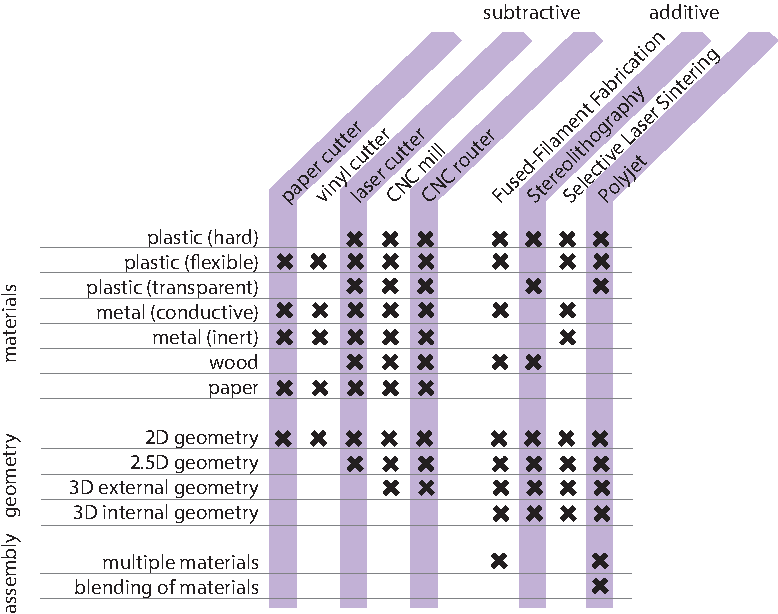
\includegraphics[width=3in]{figures/fab-properties.pdf}
\caption{The most common materials processed by digital fabrication machines, including plastic and wood, have wildly different realizable characteristics.}
\label{table:fab-properties}
\end{figure}

\subsection{Materials and Properties}

Beyond geometric properties, the types of materials that can be processed using the various additive and subtractive RP machines is equally broad. Each material lends itself to certain types of manipulations, and different materials may be more easily formed by different machines. We consider the four main types of materials used in digital fabrication for the purposes of this thesis: wood, plastic, paper, and metal.

\subsubsection{Appearance}

Materials may have a wide variety of appearance characteristics. For example, plastics can be transparent, translucent, or opaque. Paper can have color patterns or be plain white. Appearance characteristics affect the way light travels through an object.

\subsubsection{Rigidity}

A material's rigidity affords particular kinds of actions. Flexible materials can be bent, while more rigid ones do not encourage bending actions.

\subsubsection{Conductivity}

Electrical properties may allow a material to be used as a part of a circuit. Metal is the only common material that is conductive, but material mixing (e.g., plastic filament with embedded graphite, or silver ink printed on paper's surface) can lead to conductive properties in materials that lack them.

\subsubsection{Plastic}

Hard plastics---mainly thermoplastics like acrylonitrile butadiene styrene (more commonly known as ABS) and polylactic acid (known as PLA)---are the materials du jour in the maker community. They come in the form of heatable, extrudable filaments for FFF machines (e.g., Makerbot, Printrbot, Reprap, uPrint). Hard plastics can also be additively processed with other 3D printing techniques, for example photocure plastics in polyjet machines (ABS-like and Vero series for Objet machines) and SLA machines (methacrylates in Form1), or thermoset plastics like epoxy in research systems (e.g., Harvard's system \cite{compton-epoxy}).

Hard plastics can also be subtractively processed through milling and laser cutting, although many plastics are unsafe for laser vaporization (e.g., ABS plastic emits chlorine gas when lasercut).

Flexible plastics are less common than hard ones, though there are some notable materials here: thermoplastic polyurethane (sold as Ninjaflex) is a filament-style flexible material for use in FFF machines, and some polyjet machines likewise have support for flexible plastics (e.g., Tango series for Objet).

Subtractive processing for flexible plastics is possible, though may be more challenging due to different shear parameters than stiffer materials. PVC plastic in the form of vinyl sheets can be cut to shape with a vinyl cutter.

Transparent plastics are not yet available for most maker-class machines, though many SLA-processed resins are optically translucent and polyjet machines offer optically transparent plastics (e.g., VeroClear for Objet). Laser cutters are suitable for processing sheets of transparent acrylic, as well.

\subsubsection{Metal}

Conductive metal is relatively simple to process subtractively (e.g., milling circuitboards on a CNC router), even by vinyl cutters which can cut thin metal foils. Certain conductive metals, e.g., steel, can be directly laser-sintered in a high-heat process. Conductive-impregnated filaments for FFF machines do exist in limited use, but they are typically based on graphene (carbon) rather than metals. The new Voxel8 FFF 3D printer \cite{voxel8} uses a silver-based material for conductive purposes.

Inert metals are processed in essentially the same ways as conductive metals, although they have not been engineered for use in FFF filaments.

\subsubsection{Wood}

Wood-type materials are most commonly subtractively processed (e.g., by CNC routing). Newer processes are available to add wood in the form of sawdust to FFF-compatible filaments (e.g., woodfill by colorfabb), and also to laser sinter with wood chips \cite{materialise-wood}.

\subsubsection{Paper}

Paper is trivially subtractively processed. None of the four main 3D printing methods can use paper-based materials, though one subtractive/additive method uses stacks of cut paper to create 3D paper models (e.g., MCor IRIS).

\subsection{Machine Abilities}

The varying constructions and methods of additive and subtractive fabrication machines allow them to process particular materials in particular ways. We briefly describe geometric and compositional possibilities for a variety of digital fabrication techniques.

\begin{figure}
\centering
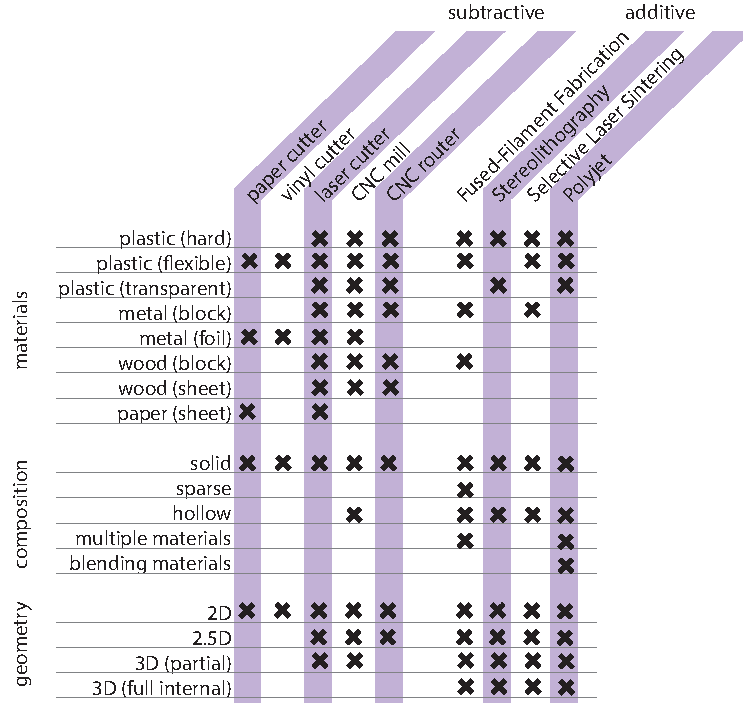
\includegraphics[width=5in]{figures/materials-machines.pdf}
\caption{Additive and subtractive RP machines each have their own sweet spots of operation. Subtractive tools can process more types of materials, but additive ones offer more compositional and geometric flexibility.}
\label{table:materials-machines}
\end{figure}

\subsubsection{Material Composition}

Additive digital fabrication methods offer significant freedom in terms of assembly methods. While subtractive machines are typically limited to the original composition of the material (material is loaded in as a solid block and parts are removed from it), additive fabrication methods can create objects which are built of solid, sparse, or hollow material (see Figure \ref{fig:composition}). These material compositions give rise to opportunities to design acoustics, airflow, or other wave/fluid systems; additionally they give a designer fine-grained control over object strength and weight.

Additive machines also permit deviation from a material's original characteristics in their ability to blend and use multiple types of stock material. This allows a polyjet machine to take as input black material and white material, and create as output either an object with both black and white material, or an object exhibiting a variety of shades of grey. Blending and the use of multiple materials allows for control of appearance, rigidity, and conductivity, as described above.

\begin{figure}
\centering
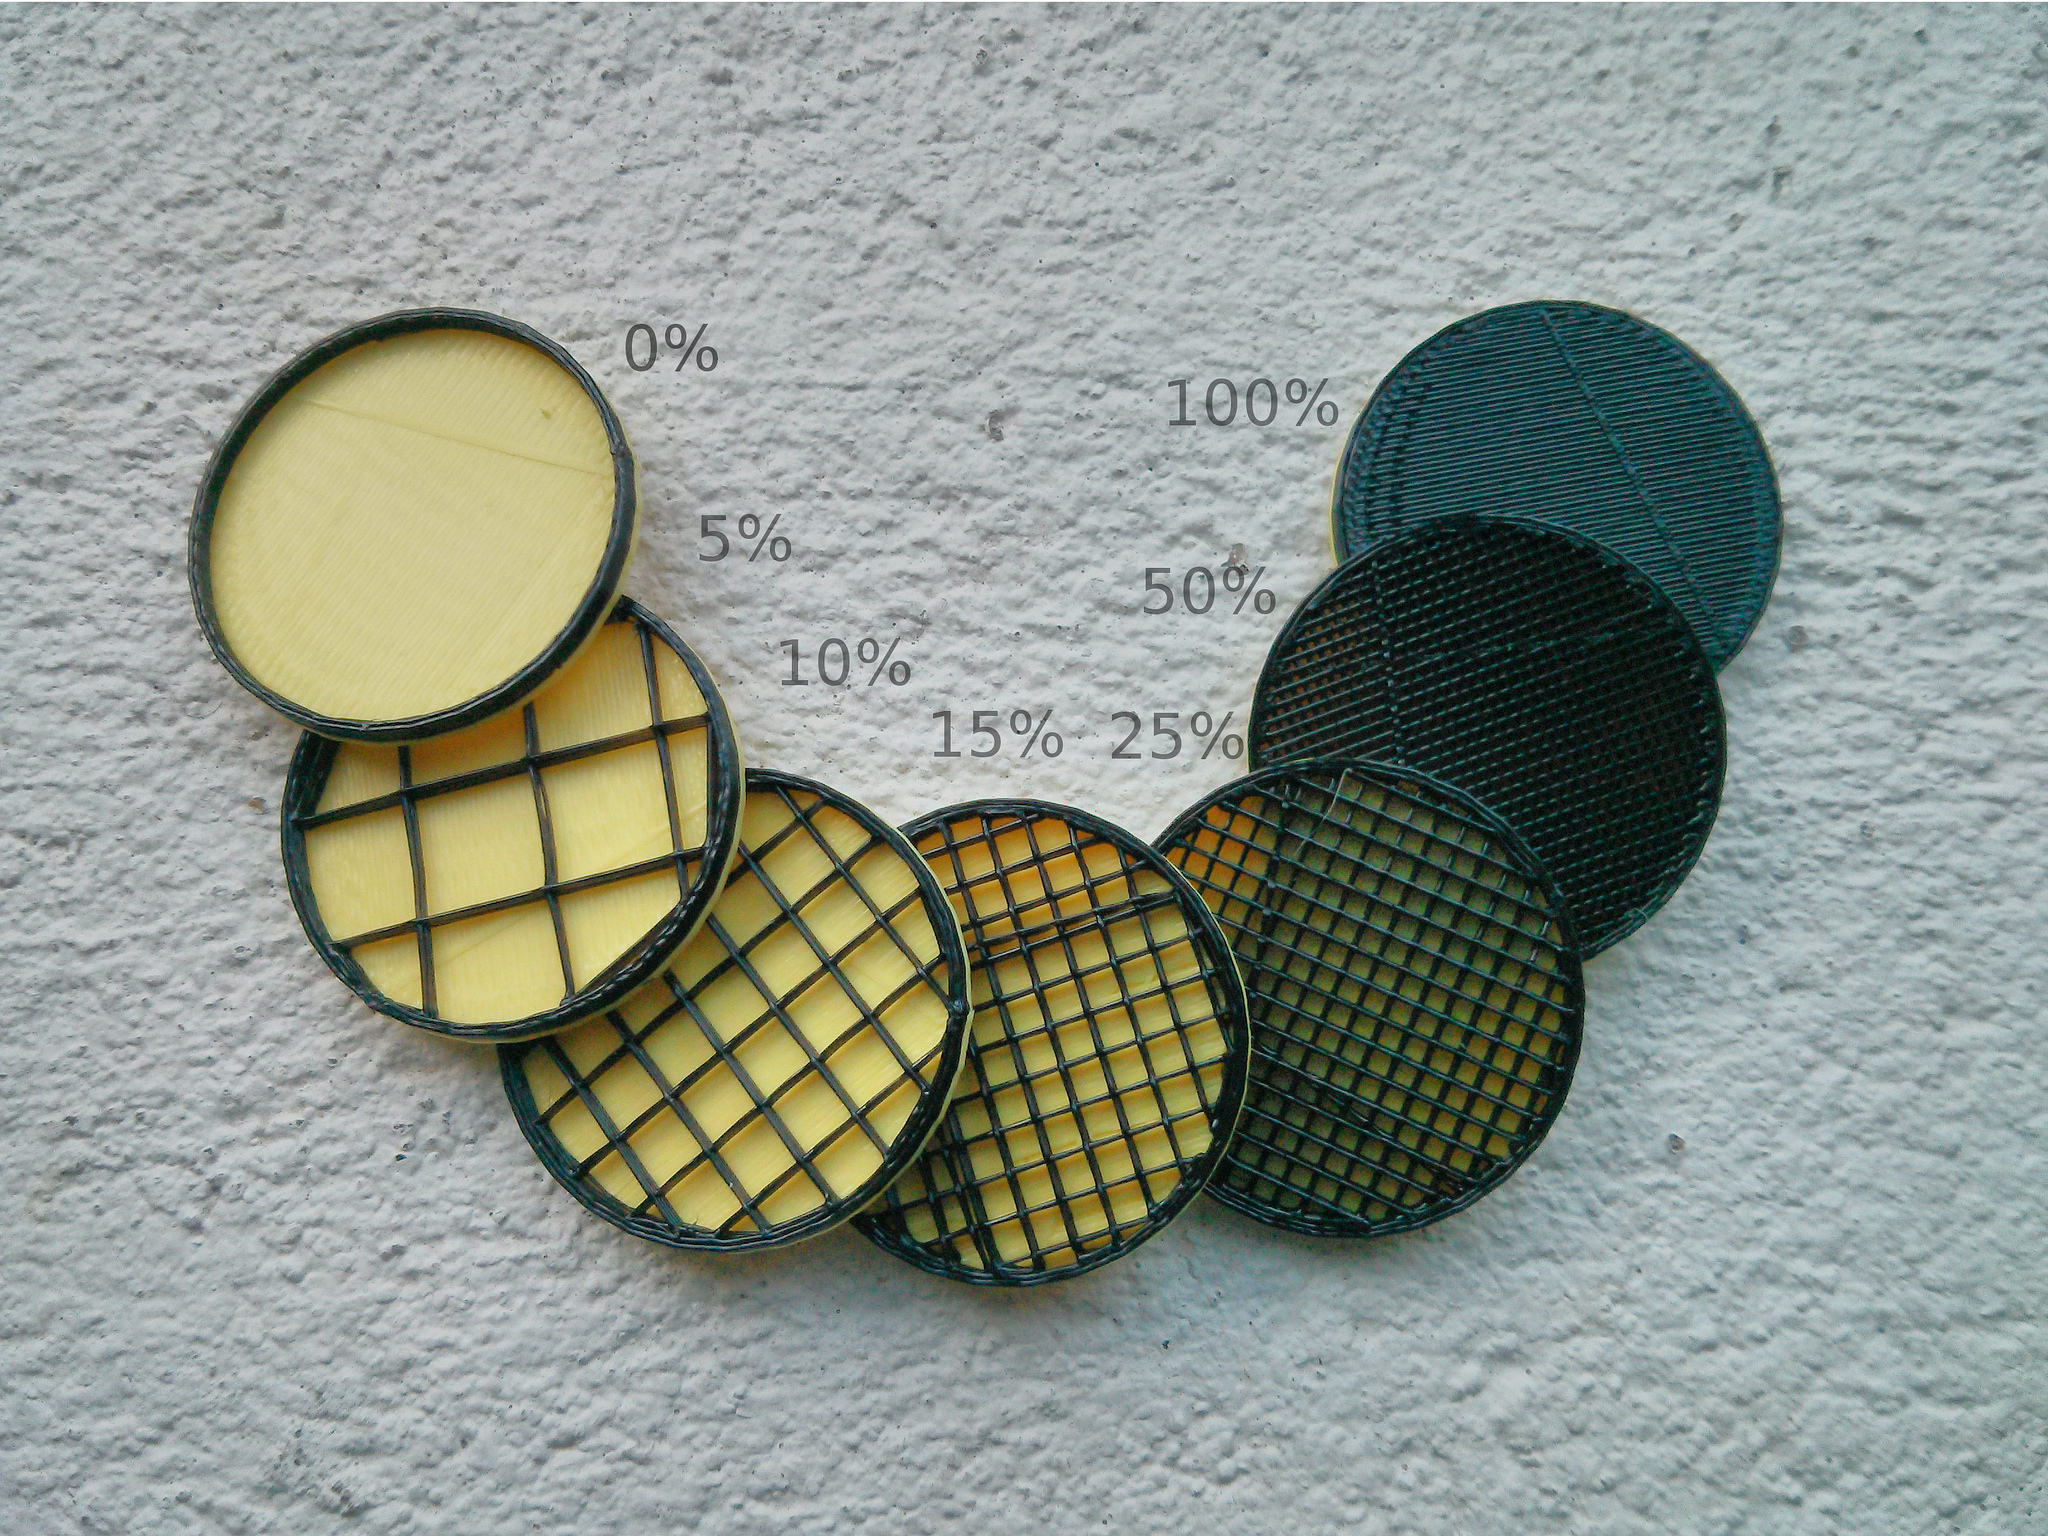
\includegraphics[width=4in]{figures/infills.jpg}
\caption{FFF machines can lay plastic to create a variety of material compositions, ranging from hollow to sparse to solid. Here, we see a variety of compositions, arranged in order of percent(material/air). (from think3d.in)}
\label{fig:composition}
\end{figure}

\subsubsection{Geometry Fabrication}

Digital fabrication machines can support any complexity of geometry, from 2D images on paper (as an inkjet printer produces) to 3D projections of 4D objects (like Shapeways's Klein bottles printed in steel) (see Figure \ref{fig:range}). We describe the possibilities for the various geometries, as well as machines that could produce them. Note that we list machines at the edge of their range: for example, a CNC mill (listed under 3D external) can also make 2.5D or 2D objects.

\begin{figure}
\centering
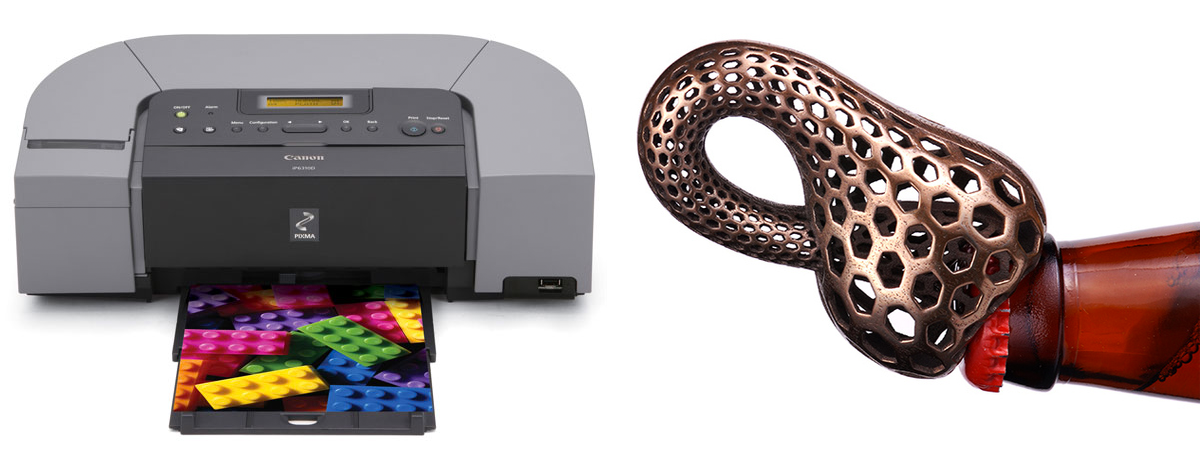
\includegraphics[width=4in]{figures/range.png}
\caption{The range of objects produceable via digital fabrication is huge: from 2D images on paper (left, from Amazon), to 3D projections of 4D objects (right, from Bathsheba on Shapeways).}
\label{fig:range}
\end{figure}

\emph{2D geometry}: 2D geometry lies flat on a surface, but can manifest as an image printed on paper, a sticker cut from vinyl, or a barcode engraved on granite. Machines that support 2D geometry fabrication include vinyl and paper cutters, as well as inkjet printers.

\emph{2.5D geometry}: A slight jump from 2D is 2.5D: a 2D shape with additional \emph{depth} information. The canonical machines to create 2.5 objects are 3-axis CNC routers, which mill away material from the surface and can take multiple passes for deeper features.

\emph{3D external geometry}: Features like overhangs can be challenging to mill using a 2.5D machine, as subtractive techniques require that the machine tool has unobstructed access to the surface to be milled. Creating such features on a 2.5D machine may require reorienting an object several times. Some machines are capable of creating arbitrary 3D external geometry, including overhangs, without manual reorientation of a part. This is can be accomplished by machines that use both a model material and a sacrificial support material: combining the two materials permits overhangs that may not be possible using only a single material. However, removal of this support material can be challenging, depending on the process used. (See \cite{savage-sot} for a more complete treatment of support material and removal techniques.) 3D printers can produce overhang geometry by laying support material as a part of each 2D object slice, and 5-axis CNC mills can produce overhangs via automatic object reorientation.

\emph{3D internal geometry}: Full control over internal geometry can only be executed via additive manufacturing, and it allows for designed cavities, mechanisms, textures, and more on the interior of objects manufactured in a single pass. Again, this is typically executed by machines that lay sacrificial support material.

\section{Single-Sensor Sensing Techniques}

One key research area in Human Computer Interaction is designing new techniques and algorithms to help computers accept human input. Thus, while many of the input techniques here could be used in, for example, machine-to-machine communication, we describe how a person's actions might create a usable control signal.

\subsection{Single-sensor Motivation}

Why use a single sensor? To reduce time spent on each iteration of a prototype performing assembly and calibration, we aim to allow users to fabricate an object and snap on a single sensing module. In the future, it would be interesting to explore multi-sensor modules (e.g., modern smartphones have magnetometers, capacitive screens, microphones, cameras, and more), however as initial work we are exploring one sensor at a time.

\subsection{Sensor Types}

A ``single sensor'' can take many forms, ranging from a humble switch which opens and closes to a high-speed video camera which captures 2D visual information at 1000Hz to an accelerometer measuring G-forces in 3 directions.
As they represent a vast array of actions sensed, physical phenomenon, and other aspects, there are multiple ways of organizing sensors for discussion purposes. We use the hierarchy proposed by the Modern Sensor Handbook \cite{fraden-modernsensors}: it arranges sensors by changes sensed, which neatly aligns with our user-driven prototypes.

The major categories in the Modern Sensor Handbook are
\begin{itemize}
    \item occupancy and motion
    \item position, displacement and level
    \item velocity and acceleration
    \item force, strain and tactile
    \item pressure
    \item flow
    \item acoustic
    \item humidity/moisture
    \item light detectors
    \item radiation detectors
    \item temperature
    \item chemical sensors
\end{itemize}

%\valkyrie{The physical effects that are the basis of sensors include: capacitance, magnetism, induction, resistance, piezoelectric effect, pyroelectric effect, hall effect, thermoelectric effect, ...}

Curious readers can learn more of their workings from the Handbook \cite{fraden-modernsensors}; we take their triggers and high-level functions to be self-evident here.

\section{Promising Overlaps}

The spaces of both material and fabricated properties, and sensors are vast: we describe some ways to think about combining them to actually fabricate sensing objects.

\begin{figure}
\centering
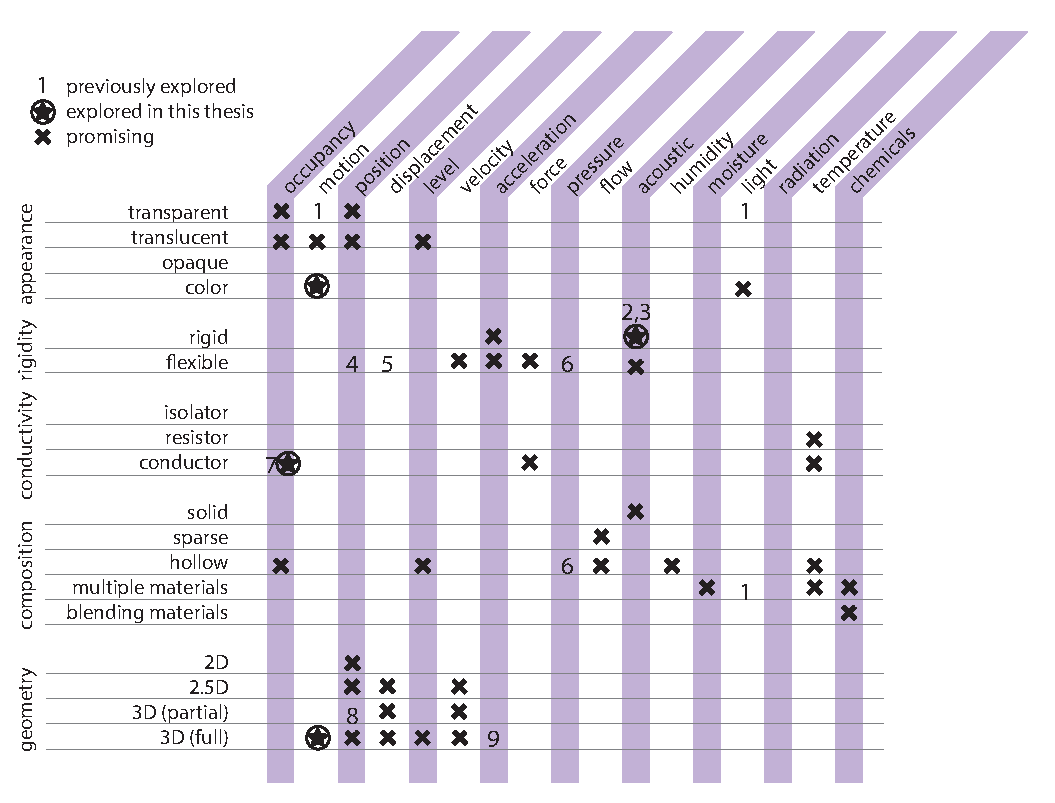
\includegraphics[width=6in]{figures/sensing-fab.pdf}
\caption{Lining up the possibilities of fabricatable properties with sensor types, we can see several areas that are promising for further exploration. We also identify pairings that have been explored previously, as well as pairings explored in this thesis. 1. Printed Optics \cite{willis-printedoptics}, 2. Acoustruments \cite{laput-acoustruments}, 3. Stane \cite{murray-smith-stane}, 4. Flexibend \cite{chien-flexibend}, 5. Dynamic latex buttons \cite{harrison-buttons}, 6. Pressure-sensing robot skins \cite{slyper-pressure}, 7. Capricate \cite{schmitz-capricate}, 8. Design by physical composition \cite{doering-composition}, 9. Making 3D printed objects interactive with wireless accelerometers \cite{hook-making}}
\label{fig:range}
\label{fig:sensing-fab}
\end{figure}

\subsection{Principles}
    
    Several principles guide our selections. Namely,
    \begin{itemize}
        \item a user's manipulating the object should generate a control signal senseable using the given sensor. For example, bending a flexible material generates a signal detectable by a displacement sensor. This may require usage of transformation mechanisms, as described above.
    
        \item the material can conduct or predictably insulate the control signal: for example, rigid materials conduct sound waves and can be used with microphone sensing, but flexible/soft materials could be used to insulate sound and direct it through an object.
    
        \item geometry should work with the sensing abilities of a given technology. For example, an object with a solid core would not admit fluids for flow sensing; 3D internal geometry or a hollow object would make this type of sensing possible.
      
        \item material composition may pair with material properties to get additional sensing. For example, \emph{blending} stiff and flexible plastics may allow for more unique degrees of sensing with a flex sensor than flexible materials alone. 
    \end{itemize}
    
    These principles give rise to the \textbf{x}s marked in Figure \ref{fig:sensing-fab}.
    
\subsection{The Most Promising Overlaps}

    While clearly several types of overlaps have been extensively explored, we suggest a couple very promising unexplored areas here.
    
    One such promising idea uses force sensors with flexible materials. As a user manipulates an input, the stretch, compression, and torque forces they generate disperse through an object. A force sensor located near the center of all inputs should be able to detect these transmitted actions. This may be easiest with polyjetted 3D printed objects, as their materials properties are the most consistent (and therefore easiest to model) due to their fine resolution.
    
    Prototype objects could be designed with translucent internal piping and gate-like structures at interaction points: the pipes, when filled with liquid, could be amenable to sensing with a camera or level sensor. This could be thought of as a liquid-state flute. Additionally, the orientation of such an object in space could be calculated using liquid levels, as they would settle based on gravitational forces.
    
    Users' bodies maintain a higher temperature than typical room temperatures. This fact could be used in an interactive object which has conductive pathways at interaction points or grip locations, leading to a temperature sensor. This type of sensing would be slower than simple capacitance sensing, but could provide additional passive cues like overall body temperature or time spent in a particular configuration. To properly sense, such an algorithm might require knowledge of the interacting human's temperature in addition to digital geometry knowledge.
    
\subsection{Overlaps Discussed in this Thesis}

    \subsubsection{Conductive Metal + 2D Geometry + Capacitive Sensor}
    
    Chapter 4 describes Midas, a technique for creating custom capacitive touchpads CNC cut from adhesive copper foil. These can be affixed to everyday objects and sensed using a single capacitive touch controller.
    
    \subsubsection{Hard Plastic + 2D/3D Geometry + Microphone}
    
    Chapter 5 describes Lamello, a technique for creating tines from hard plastic; when struck each tine vibrates at a characteristic frequency which can be classified using a microphone.
    
    \subsubsection{Multi-color + 3D Internal Geometry + Camera}
    
    Chapter 6 describes Sauron, a technique leveraging colored arbitrary internal geometries to create mechanical input devices that can be sensed by a single embedded camera.